\documentclass[12pt]{article}
\usepackage{graphicx}
\textwidth 17cm
\oddsidemargin -0.54cm  %2cm Rand links
\topmargin 0.46cm %3cm Rand oben
\headheight 0cm % no header
\headsep 0cm
\textheight 22cm
\parskip 6pt
\parindent 0pt

\newenvironment{mylist}
  {\begin{list}{$\bullet$}{\parsep 0pt}}
  {\end{list}}
\newenvironment{mysublist}
  {\begin{list}{$-$}{\parsep 0pt \topsep 0pt \leftmargin 2cm}}
  {\end{list}}
\newcommand{\degree}{\mbox{$^{\circ}$}}
\newcommand{\see}{\mbox{$\rightarrow$}}

%\newcommand{\pending}[1]{\noindent \fbox{\parbox{\textwidth}{\em #1}}}
%\newcommand{\error}[1]{\noindent \fbox{\parbox{\textwidth}{\sf #1}}}
\newcommand{\pending}[1]{\noindent \fbox{ \em #1}}
\newcommand{\error}[1]{\noindent \fbox{ \sf #1}}

\newcommand\todo[1]{$\Longrightarrow$ {\em #1} }


\begin{document}\noindent

\parbox[t]{0.7\hsize}{
  {\Huge\bf OPA User Guide} ~~version {\bf 4.047} \\
  Andreas Streun, PSI, \today
} \hfill  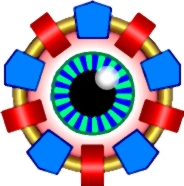
\includegraphics{opalogo_small.jpg}
\rule{\hsize}{1pt}
\section{Introduction}
OPA's main purpose is to support the development of electron (positron) storage rings. Emphasis is on visualization and interactivity.

OPA is in particular useful for designing high brightness light source lattices, but may be used for transfer lines and other types of lattices as well.

OPA uses simplified models and approximations in order to support straightforward design work. Results should be checked with other codes using more complete beam dynamics models.

For the beam dynamics implemented in OPA see the accompanying document ``inside OPA''. To get started try ``OPA tutorial''. 
In this document we try to give a complete overview on data and function of OPA. While reading you may have the two other documents within reach and OPA running.

\subsection{History and acknowledgements}
OPA is based on the code OPTIK from Klaus Wille,
who started in the 80's already to work on a design tool for electron rings.
In 1993 he kindly passed it on to the author, who developed it further
and used (and uses) it for the design of the Swiss Light Source, SLS (and the upgrade, SLS-2).
Algorithms for sextupole optimization and signal processing were kindly contributed by Johan Bengtsson.
Simon Leemann did a lot of tests and suggested many extensions and changes during the design of MAX-IV. Michael Borland and Chun-xi Wang tested the module for non-linear optimization for consistency with the ELEGANT code and helped to find several bugs. Volker Ziemann helped with implementation of coupling and calculation of radiation integrals.

\subsection{Capabilities and limitations}
OPA includes the following features:
\begin{mylist}
\item Human readable lattice input/output and robust lattice reader.
\item Text editor and modular editor for variables, elements and segments.
\item Interactive graphical design of linear optics with many convenient functions as knobs, zoom, matching, tune diagram etc.
\item Implementation of the Edward-Teng formalism for coupled betatron motion (not all modules).
\item Interactive optimization of sextupole and octupole Hamiltonian in $1^{\rm st}$ and $2^{\rm nd}$ order.
\item Tracking with FFT: Poincar\'e plots, resonance guesses and amplitude dependent tunes.
\item Tracking of dynamic apertures.
\item Tracking of Touschek lifetime.
\item Correlated misalignments
\item Display of lattice geometry.
\item Orbit distortion and correction.
\item Simulation of the injection process.
\item Calculation of magnet currents and export of EPICS snap files.
\item Export of TRACY-2, TRACY-3, MAD-X, ELEGANT and BMAD lattice files.
\end{mylist}

OPA has the following limitations:
\begin{mylist}
\item Only correct for rings with large circumference and high energy:
\begin{mysublist}
\item High relativistic approximation: $\gamma \gg 1$
\item Paraxial approximation: $x' = dx / ds \ll 1$
\item Large curvature approximation: $x \ll \rho$ (bending magnet radius)
\end{mysublist}
\item Exactly correct only on energy (i.e. $\Delta p/p = 0$),
since it uses internally $x'$  instead of the canonical coordinate $p_x$.
\item Nonlinear elements are treated by a $2^{\rm nd}$ order symplectic integrator only.
\item Only planer insertion devices allowed. Simple model as dipole array.
\item Only 4D tracking (no synchrotron oscillations).
\end{mylist}

\section{Installation}
OPA started in Borland Turbo Pascal, was converted to Borland Delphi, and then to Lazarus Free Pascal, which is like an open source version of Delphi. 
Lazarus is platform independent. Presently OPA runs on Windows-10 and on xUbuntu with GTK2. Both versions are built from the same source files.

In W10 Lazarus creates a single executable {\tt opa.exe}, which can be downloaded and should run on any W10-system.
In Linux an executable {\tt opa} is created, but it only runs on the system where it was created. A debian file
to install the program and set the dependencies has not yet been established. Instead one has to use Lazarus to build the executable from the source.

\todo{to do: create a debian file to install on Linux.}

W10-executable, source files and documentation is availble at the OPA page {\tt ados.web.psi.ch/opa}. 

For using OPA it is recommended to create a folder for lattice data, probably with subfolders for different projects. The executable should be in a separate program folder. If the executable is built from Lazarus, it is usually a subfolder named {\tt /lib/x86\_64-linux} or {\tt -win64} under the folder where the source files are located.
Note, that OPA needs write permission for the folder
where the executable is located in order to write two settings files, named {\tt opa4\_glob.ini} and {\tt opa4\_path.ini}

\todo{This should be improved to make a clear separation between the program files and the user files changed at run-time.}

When starting OPA, it will write a settings files {\tt opa4\_set.ini} in each data folder selected in order to remember settings for the next session. These settings can be different for each data folder. The file {\tt opa4\_path.ini}, which exists only once in the executable's folder, remembers the path names of the the last used files.

OPA lattice files are named {\tt *.opa}. Unlike many other lattice codes, these files are not read-only but can be composed in OPA and saved. OPA can start from scratch without reading a lattice files.
Many more files, to be described below, are exported by different modules on request during the sessions. 


\section{Lattice Data}
Lattice {\bf elements} are of different type, like quadrupole, drift space, dipole etc. 
A lattice is a line-up of elements, called a {\bf segment}. Segments may contain a mixture of other segments and elements, thus the lattice is made from nested segments to be unpacked recursively in order to get an array of elements to work with.

An element has a {\bf name}, a {\bf type} and a set of {\bf parameters} depending on the type.
Parameters  may be numbers (of different type like integer, real, boolean etc.) or strings representing an algebraic expression. Expressions may contain {\bf variables}, which are either numbers or expressions themselves.~--
Consider this simple example:

{\small \begin{tabular}{ll}
{\tt V1 = 0.5;}  & A variable given as number \\
{\tt V2 = -2*V1;}  & A variable given as expression \\
{\tt D: Drift, L=1.0;} & A drift space of length 1m \\
{\tt Q1: Quadrupole, L=0.2, K=V1;} & Quadrupole length 0.2 m, strength $0.5\,$m$^{-2}$ \\
{\tt Q2: Quadrupole, L=0.2, K=V2+0.1;} & Quadrupole, strength $-0.9\,$m$^{-2}$  \\
{\tt B: Bending, L=0.5, T=10, T1=5, T2=0;} & Dipole of angle 10\degree, entry/exit edge angles 5\degree/0\degree \\
{\tt S1: B, D, Q1;} & a segment connecting dipole drift, quadrupole\\
{\tt S2: D, -S1, 2*D, Q2;} & segment with inverted segment and repeated elements.\\
$\Longrightarrow$ {\tt D, -Q1, -D, -B, D, D, Q2;} & this would be the expanded lattice.
\end{tabular}
}

Note that both quadrupole strengths depend on the variable {\tt V1} which will be a ``knob'' in OPA and thus they are varied in a correlated way. Elements and segments can be repeated or inverted. For most elements, inversion does not change their properties, but in case of a bending magnet, edge angles are interchanged.

\todo{Expressions are not allowed for all element parameters, presently only for length, quad strength, bending and edge angles) however this would the straightforward to extend to all.}\\

Lattices are read from and written to {\tt *.opa} lattice files. The syntax, as indicated above, is rather simple and similar to lattice files for other codes like TRACY or MAD (check out an example file or the tutorial).

First come a few global parameters, \see\ref{ssecglo},
then comes the list of variables, \see\ref{ssecvar}, then the list of elements, \see\ref{ssecelem}, and finally the list of segments, \see\ref{ssecseg}, which will
be unpacked recursively to generate the lattice.

All inputs are optional, since OPA may start without lattice as well.
For parameters of an element not given in the input file, OPA assumes reasonable defaults.
If a parameter is mistyped, OPA will ignore it and set it to the default value.

Text in curly brackets { \tt \{ ... \} } is treated as comment,
i.e. ignored by OPA, except text bracketed by {\tt \{com ... com\}},
which is the "official" comment text like lattice title and some notes.
Further comments visible in the {\tt *.opa}-file are generated by OPA
for the user's convenience. Comments written manually into
the {\tt *.opa} file will be lost.

All input lines (defining an element, a segment), which may extend over several physical lines in the file, have to be terminaed by semicolon ({\tt ;}).

\subsection{\label{ssecglo}Global Parameters}
The lattice header includes the offical comment {\tt \{com ... com \}},
the beam {\tt Energy} in GeV (default 1~GeV) and a flag {\tt Rotinv=0/1;} telling if rotations are inverted too if an element is inverted (depending on the application the one or the other option is preferable.)

Further the initial optical parameters ({\tt BetaX=...} etc.) at the beginning of the last used segment are written to the file header.
\todo{This has historical reasons and should be removed and replaced by an OpticsMarker (see below).}

To use the option of exporting magnet currents and channel names (\see\ref{sseccur}), a
link to the corresponding allocation and calibration files is required
and should be given at the beginning of the {\tt *.opa} file:\\
{\tt allocation  = (allocation-file).dat; calibration = (calibration-file).dat; }
See {\tt ados.web.psi.ch/slsdesc/optic/magnets.html} for SLS allocation (lookup) and calibration files.


\subsection{\label{ssecvar}Variables}
Variables can be defined to be referenced by each other or by some of the elements.
Variables can be numbers of expressions using basic operators ({\tt +-*/}) and arbitrary number of bracket pairs. Variable name has to start with a character, then numbers and characters may follow. Syntax check is performed. Example: {\tt A = 0.5; XB3S = (1.0-A)/2; }\\

\subsection{\label{ssecele}Elements}

Tables \ref{tabel1} and \ref{tabel2} list the parameters of the elements: column ``in file'' tells how to adress them in the lattice file (case insensitive), column ``in record'' refers to OPA's internal {\tt ElementType} record (in unit {\tt OPAGlobal.pas}). 
An asterisk indicates that an algebraic expression is allowed too. In this case the record contains a string of same name followed by {\tt \_exp}. ``unit'' is the physical unit for the number in the lattice file. ``note'' refers to a comment below.
The element parameters can be accessed interactively from the OPAEditor menu as well.

\begin{table}
\caption{\label{tabel2}Element description, part I}\vspace{1em}
\begin{tabular}{lllcr}
Property & in file & in record & unit & note \\
\hline
\multicolumn{5}{l}{{\bf All elements}}\\
Name	& & {\tt nam} & & \\ 
Length		& {\tt L} & {\tt l*} & m & \\
Apertures & {\tt Ax, Ay} & {\tt ax, ay} & mm & a) \\
Rotation & {\tt Rot} & {\tt rot*} & \degree & b) \\
\hline
{\bf Drift} & {\tt Drift} & {\tt cdrif} & & \\
(protect) & {\tt Block} & {\tt block} & -/- & c) \\
\hline
{\bf Quadrupole} & {\tt Quadrupole} & {\tt cquad} & & \\
Strength & {\tt K} & {\tt kq*} & m$^{-2}$ & \\
\hline
{\bf Bending magnet} & {\tt Bending} & {\tt cbend} & & \\
Deflection & {\tt T} & {\tt phi*} & \degree & d) \\
Edge angles & {\tt T1, T2} & {\tt tin*, tex*} & \degree & \\
Focusing strength & {\tt K} & {\tt kb*} & m$^{-2}$ & \\
Full gap & {\tt Gap} & {\tt gap} & mm & \\
Edge K1 & {\tt K1, K1in, K1ex} & {\tt k1in, k1ex} & 1 & e) \\
\hline
{\bf Combined function} & {\tt Combined} & {\tt ccomb} & & f) \\
Deflection & {\tt T} & {\tt cphi*} & \degree & d) \\
Edge angles & {\tt T1, T2} & {\tt cerin*, cerex*} & \degree & \\
Focusing strength & {\tt K} & {\tt ckq*} & m$^{-2}$ & \\
Full gap & {\tt Gap} & {\tt cgap} & mm & \\
Edge K1 & {\tt K1, K1in, K1ex} & {\tt ck1in, ck1ex} & 1 & e) \\
Sextupole strength & {\tt M} & {\tt cms} & m$^{-3}$ & g) \\
(slices) & {\tt N} & {\tt cslice} & 1 & h) \\
\hline
{\bf Sextupole} & {\tt Sextupole} & {\tt csext} & &  \\
Sextupole strength & {\tt K} & {\tt ms} & m$^{-3}$ & g)i) \\
(slices) & {\tt N} & {\tt sslice} & 1 & h) \\
\hline
{\bf Thin multipole} & {\tt Multipole} & {\tt cmpol} & &  \\
Multipole order & {\tt N} & {\tt nord} & 1 &  \\
Integrated strength & {\tt K} & {\tt bnl} & m$^{1-n}$ &  g) \\
length & {\tt Lmag} & {\tt lmpol} & m & j) \\
\hline
{\bf Undulator} & {\tt Undulator } & {\tt cundu} & &  k)\\
Period length & {\tt Lamb} & {\tt lam} & mm &  \\
Peak field & {\tt Bmax}&  {\tt bmax} & T & \\
Full gap & {\tt Gap} & {\tt ugap} & mm & \\
Fill factors & {\tt F1,2,3} & {\tt fill1,2,3} & 1 & l) \\
(half) & {\tt Half} & {\tt halfu} & -/- & m) \\
\hline
\end{tabular}
\end{table}

\begin{table}
\caption{\label{tabel1}Element description, part II}\vspace{1em}
\begin{tabular}{lllcr}
Property & in file & in record & unit & note \\
\hline
{\bf Kicker} & {\tt } & {\tt ckick} & &  \\
Multipole order  & {\tt N} & {\tt mpol} & 1 &  \\
Peak field offset  & {\tt X} & {\tt xoff} & mm & n)  \\
Int. strength $\leftrightarrow$ peak kick & {\tt Amp} & m$^{1-n}$ $\leftrightarrow$ mrad & \\
Period & {\tt T} & {\tt tau} & ns & o) \\
Delay & {\tt Delay} & {\tt delay} & ns & o) \\
(slices) & {\tt NK} & {\tt kslice} & 1 & \\
\hline
{\bf Septum} & {\tt } & {\tt csept} & &  \\
\multicolumn{5}{l}{(not yet implemented)} \\
\hline
{\bf Solenoid} & {\tt } & {\tt csole} & &  \\
Strength & {\tt K} & {\tt ks} & m$^{-1}$ &  \\
\hline
{\bf Hor. corrector} & {\tt H-corrector} & {\tt ccorh} & & p) \\
Kick & {\tt Dxp} & {\tt dxp} & mrad &   \\
\hline
{\bf Vert. corrector} & {\tt V-corrector} & {\tt ccorv} & &  p) \\
Kick & {\tt Dyp} & {\tt dyp} & mrad &   \\
\hline
{\bf BPM} & {\tt Monitor } & {\tt cmoni} & &  p) \\
\multicolumn{5}{l}{ --~no parameters to set~-- }\\
\hline
{\bf Girder} & {\tt } & {\tt cgird} & &  \\
Type & {\tt typ} & {\tt gtyp} & 1 &  q) \\
Shift & \multicolumn{4}{l}{(not implemented)} \\
\hline
{\bf Optics marker} & {\tt } & {\tt comrk} & & r) \\
Orbit & {\tt OrbitX/Y,OrbitXp/Yp} & {\tt om$^{\wedge}$.orb[4]} & mm, mrad & \\
Normal mode betas & {\tt BetaX/Y, AlphaX/Y} & {\tt om$^{\wedge}$.bet[4]} & m, 1 & \\
Dispersion & {\tt EtaX/Y, EtaXp/Yp} & {\tt om$^{\wedge}$.eta[4]} & m, 1 & \\
Coupling matrix & {\tt C11, C12, C21, C22} & {\tt om$^{\wedge}$.cma[4]} & m, 1, m$^{-1}$ & \\
(screen) & {\tt Screen} & {\tt screen} & -/- & \\
\hline
{\bf Photon beam} & {\tt PhotonBeam} & {\tt cxmrk} & &  s) \\
Length & {\tt XL} & {\tt xl} & m & \\
Style & {\tt Style} & {\tt nstyle} & 1 &  \\
\hline
\end{tabular}
\end{table}

Comments to the tables:

a) a rectangular aperture $(\pm a_x)\times(\pm a_y)$ is assumed for aperture checks in tracking, however an elliptic aperture (half axes $a_x$, $a_y$) is assumed for calculation of linear acceptance and for Coulomb lifetime.

b) positive rotation is counter-clockwise around the beam direction, i.e. 90\degree rotation of a dipole will deflect the beam upwards.

c) if keyword is present, the drift is shown as grey solid, not invisible; useful to indicate protected space, e.g. coils of a magnet.

d) Positive deflection is towards the ring center, i.e. in $-x$-direction and thus will create positive dispersion.

e) $K_1$ is the fringe field parameter defined by Brown (see ``inside OPA''/Elements/on-axis). If only {\tt K1} is given in the lattice, the same parameters is applied to both edges. 

f) ``Bending'' and ``Combined'' are almost identical, except that ``Combined'' allows a sextupole component. This has historical reasons. \todo{to be merged in one element.}

g) Multipole definition includes the factorial, i.e. $b_n = \frac{p}{e}\frac{1}{(n-1)!}\frac{d B^{(n-1)}_y}{d x^{n-1}}$

h) Internally the thick, nonlinear magnet is approximated by $N$ slices of length $L/N$ with a thin multipole of integrated strength $b_nL/N$ at the center.

i) If sextupole length is given as zero, the strength is integrated strength, unit m$^{-2}$.

j) Multipole is always considered thin. If a length {\tt LMAG} (not {\tt L}!) is given, it just reserves spaces of {\tt LMAG/2} on both sides of the single, thin kick.

k) Helical undulators are not (yet) implemented, only planar undulators are supported.

l) Undulator fill factors used for fast calculation of radiation integral (see ``inside OPA`` sec.3), depending on the field variation over a period. Default is sinusoidal field. 

m) Internally, an undulator is modelled as a series of small dipoles, where the dipoles at entry and exit are attenuated to $1/4$ and $-3/4$ field of the inner array dipoles. The keyword {\tt half} suppresses the attenuation at the exit, because sometimes one likes to split the undulator {\tt(U)} to insert a marker {\tt(M)}. In this case the full undulator is modeled from two halfves as {\tt(U,M,-U)}.

n) For {\tt X=0} the kicker is considered a pure multipole kicker and {\tt K} gives its integrated strength. Non-zero {\tt X} identifies a non-linear kicker with $\sin^{n-1}(2\pi x/X)$ shaped field, and {\tt K} is the maximum kick in mrad at {\tt X}. For a dipole kicker {\tt (N=1)} the field shape is the same for both cases, and {\tt K} is the kick in mrad.

o) The pulse is assumed to be of half-sine shape with length ($=$ half period) {\tt T}, starting/ending at {\tt Delay $\pm$ T/2}. Beam time of flight is counted from the start of the lattice, and the delay has to be adjusted appropriately to kick the beam (the injection module provides a synchronization button).

p) Correctors with reserved names {\tt CH}, {\tt CV}, and monitors with name {\tt MON} are considered components of the orbit correction system, will be expanded into a series of individual elements and set by the orbit correction procedure. In the lattice a series of elements named {\tt CH001, CH002 ...} will appear, but these are not saved to the file, since they do have design values but will be set by orbit correction. The same is true for skew quadrupoles with reserved name {\tt
CS}. \\
\todo{However, OPA does not yet contain a coupling correction scheme but values are temporarily imported from a TRACY run  ({\tt Extra $\rightarrow$ test)}.}

q) The girder element defines the begin or end of a girder, thus they should appear always in pairs. Type 0 is a loose end, type 1 is a ``train link'', i.e. a [virtual] joint to the next girder, type 2,3 are secondary girders sitting on top of primary girders, where the roll of the primary girder is transmitted for type 3, but not for type2 For example the SLS dipoles bridge the girders, with 2 contact points (type 3) on one girder, and 1 contact point (type 2) on the other girder.

r) OpticsMarkers are useful for building a lattice and matching. They are markers in the lattice which on request save all 16 transverse optical parameters defining the beam (orbit, beta functions, dispersions and the coupling matrix), and which can be used as starting point for optics calculations or target points for matching. The keyword {\tt screen} indicates an optical screen to be indicated in the geometry layout.

s) Presently photon beam is only used for plotting x-ray beams in the geometry layout. There are 3 different styles (0,1,2) which can be used for different source types.

\subsection{\label{secsegm}Segments}
A segment is a line-up of elements and segments.
Many segments may be defined, the segment to be used to built the lattice is selected interactively later.
A minus sign reverses the segment. A factor repeats it.

The order of segments does not matter, so a segment used by another segment may appear later in the file.
A test is performed for circular references, which are not allowed of course.

The string {\tt nper=n} appearing somewhere in a segment line-up defines the periodicity,
i.e. the factor {\tt n} is applied for convenience to tunes, sextupole terms
etc of the lattice buit from this segment, e.g. {\tt ARC : HALF, XXX, -HALF, nper=6;}

Note: if one likes to split a bend, for example to put a marker in the centre,
and a non-zero gap is given, then one has to set {\tt K1EX=0.0} otherwise the
internal edge where the dipole is split, will have an effect on the vertical focusing!


\begin{figure}[htb]
\centering
\label{figmain}
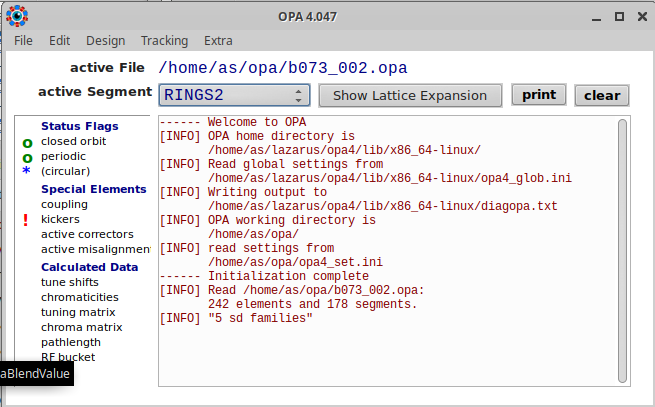
\includegraphics[width=0.7\textwidth]{mainmenu.png}
\caption{OPA main menu on xubuntu}
\end{figure}

\section{OPA functions}
For getting started, one may try the tutorial. 

The OPA menubar (see Fig.\ref{figmain}) gives access to all functions. If functions are not available, because a prerequisite is
missing (e.g. periodic solution for tracking) the items are disabled and shown in gray.
The table gives an overview of the functions behind the menubar (arrow $\rightarrow$ leads to a sub-menu, items in (brackets) are only temporary or tests):

\begin{tabular}{||l|l|l|l|l||}
\hline
File & Editor & Design & Tracking & Extra \\
\hline
New & Text Editor & Linear Optics & Phase Space &  Magnet parameters \\
Open & OPA Editor & Off Momentum & Dynamic Aperture & Magnet currents \\
Last Used $\rightarrow$ & & Non-linear & Touschek Lifetime &  (test)\\
Save & & Orbit Correction & &  (BD pattern) \\
Save as & & Injection Bumps &  & (spectra) \\
Export to $\rightarrow$ & & RF Bucket View & & Output $\rightarrow$ \\
Exit & & LGB optimizer & & \\
 & & Geometry Layout & & \\
\hline
\end{tabular}\vspace{1ex}

``Active file'' shows the selected lattice file ({\tt *.opa}). 
The ``active segment'' is selected from the segment list on the GUI.
From this segment, the {\bf lattice} is built by recursive expansion
of the segments to get the elements line-up, which is shown in the message
window when pressing ``show lattice expansion''.\\

The small window (left) indicates lattice status, if special elements are present and which data have been calculated for internal transfer between modules. The large logging window is for general status information and error messages. It may be cleared or saved to a file named {\tt LogPrint.txt}.


\subsection{File}
Here are the usual file operations. 

{\tt New} erases all saved lattice information to start composing a new lattice from scratch.

{\tt Open} reads a lattice file. Usually this is an {\tt *.opa} file. Also lattice files for other codes can be read, including files for TRACY {\tt(*.lat)}, MAD {\tt (*.mad, *.seq)}, ELEGANT {\tt (*.lte)}. However this works partially only but nevertheless may be useful to reduce manual conversion work.

{\tt Last Used} opens a list of up to 10 files used recently. Selecting one will switch to the corresponding folder and red the local {\tt opa4\_set.ini} file to restore the settings for this folder.

{\tt Save, Save as} write a {\tt *.opa} lattice file.

{\tt Export to} writes lattice files for TRACY-2, TRACY-3, MAD-X, ELEGANT, BMAD. Only a basic file is exported and some inspection/editing may be required before running the other code. If OPA Elements or element properties cannot be exported, a corresponding comment is inserted in the exported file. Note that TRACY-2, MAD-X and BMAD do not correctly invert segments containing bending magnets with unequal edge parameters: if an inverted segments contains such a bending magnet, the edge properties have to be interchanged at each (of perhaps many nested) segment inversions. Therefore, for these codes, an inverted segment is generated together with the original one to avaoid this problem. Other pecularities include using rad or degrees for angles, defining multipole strengths without or with the factorial etc. 

The sixth option in the submenu {\tt OPA (novar)} writes an opa-file replacing all variables by values. This is sometimes useful to make properties directly accessible, which are connected by variables.

{\tt Exit} closes OPA after writing the local settings to the local {\tt opa4\_set.ini} file and some global settings and the list of last used files to {\tt opa4\_glob.ini} and {\tt opa4\_path.ini} in the folder of the executable.


\subsection{Edit}

There is the OPA editor and the text editor.
New users may prefer the OPA editor, advanced users the text editor.

{\tt TextEditor} shows the file exactly as it will be saved to disk,
The ``test'' button performs a syntax check. 

{\tt OPAEditor} shows two lists, one for variables and elements, and one for segments. 
Further, there are some fields and buttons to
\begin{mylist}
\item enter the beam energy in GeV,
\item enter the global comment to be saved with the lattice file
\item set the element apertures. If the box ``set all'' is checked, all elements will be set, otherwise only elements where the apertures are larger than the new values in the two input fields,
\item enter a number for the magnet pole radius, which is used to show pole profiles and calculate fields and gradients,
\item invert all dipole polarities, if needed, and
\item expand undulator elements in explicit series of drifts and dipoles.
\end{mylist}

Clicking into the left table ``Elements and Variables'' opens a menu for the selected element or variable. If the elements is a linear magnet (quad, bending, combined), the field profile is calculated and plotted using the magnet pole radius number mentioned above. Variables and elements can be edited giving number values or algebraic expressions.

Clicking into the right table ``Segments'' opens a grid to edit the line-up of elements and segments in the selected segment. Insert and delete keys may be used. Undefined elements are shown in red, before
saving the segment they need either to be deleted or to be defined using the element editor. The periodicity field stores a number of repetitions of the segment, for example used to calculate tunes etc.

If the name of an element is changed, its entry in all segments will be changed too.


\subsection{Design $\longrightarrow$ Linear Optics}

The lattice structure appears on the optics panel main window, and a start menu pops up:

``periodic'' will try to find a solution with same parameters at both ends. If the box ``coupling'' is checked, calculations are performed for normal mode beta functions using the 4D Edward-Teng formalism, otherwise the simple 2D formalism is used, which, of course is wrong if there is a coupling element. Often, for nonzero coupling, there are two solutions for the periodic normal mode betas with interchanged tunes. Clicking the ``flip'' box shows the other solution.

``symmetric'' will try to find solution with $\alpha_x=\alpha_y=\eta'=0$
at both ends, so appending the mirror image makes it periodic. 
\todo{this option is not fully implemented and should be avoided.}

``single pass''  calculates the optics starting at its left (``initial'') or
right (``final'') end or from one of the ``optics markers'' if there are any in the lattice.
The start value for the optics calculations may be edited with the tabs at right to manually enter orbit, [normal mode] betas, dispersions [and the coupling matrix].

If periodic or symmetric solution fails, the single pass solution from initial (left)
values is calculated. If a periodic solution was found, the tune diagram pops up, see \ref{ssectun}.\\

The main window will show the optical functions:
By default, [normal mode] betas and the dispersion will be shown ($\beta_x$ in blue, $\beta_y$ in red, $\eta_x$ in green and $\eta_y$ in fuchsia). The table at right gives in its upper part
total values of the lattice (some of them only valid, of course, if the lattice would
be repeated periodically). In the lower part, local optics values are displayed.
The location can be selected by right-clicking on the plot.

The element line-up is shown at the bottom of the figure. If variables have been defined, they will appear as yellow boxes under the plot. If a variable depends on other variables, it is shown in pale yellow.

Moving the mouse over one of the elements displayed at the bottom of the figure shows its name. Left-click on an element or on a variable and releasing the mouse button after moving to one
of the "knob" fields, connects the variable or the most important parameter of the element (e.g. length of drift, strength of quadrupole etc.) to the knob. If the variable or the element parameter value is no number but an expression linking it to one or more variables, the knob only displays the value but cannot change it. So only variables and element parameters, which are pure numbers, can be varied using then knobs.

Variation of values by moving the knob slider or entering numbers changes the
optics. The range of variation is given by the fields at the bottom of the knob, which
are adjusted automatically, but can be changed using the "$<>$" and "$><$" buttons.

Left double-click on a variable or element opens the same panel as {\tt OPAEditor},  which allows
all parameters to be changed. However, element parameter expressions cannot be changed here but only in the editors.

Zoom and shift buttons at the top of the plot window magnify a region of interest: calculation through elements
proceeds in slices of maximum length corresponding to 1~pixel on screen. The plot range is adjusted automatically or by the Betafunction/Dispersion scaling buttons, depending how the ``auto/fixed'' is set. 
The ``save'' button saves curves as references and displays them in darker color. The ``clear'' buttons clears the reference.\\

The ``PlotMode'' button opens a panel to select different plots:

``Beta functions and dispersion'' is the default. The panel can be used to fix the plot range and to select what to show in the lower and upper part of the window: by default the normal mode betas are shown. Alternatively or in addition, the projections of the normal modes to the horizontal and vertical (dashed line to $x,y$ and dotted line to $y,x$) can be shown. (Without coupling, the normal mode is identical to $x,y$ and its $y,x$ projections are zero.) A third option shows the normal mode betas after each element calculated from the periodic solution of the one-turn matrix taken at this location. However, this requires to first press the button ``pp'' in the start menu~-- in a large lattice, this calculation may take quite long! The results are shown in darker color and with not interpolation.
Further one can select to show the dispersion (default), or the determinant of the coupling matrix or the orbit.

``Envelopes'' shows orbit and 1-sigma beam sizes along the lattice. It may be calculated using the equilibrium emittance from the radiation integrals or manually input values. In a coupled lattice, usually both emittances are non-zero, in the ideal case without coupling, a value may be given for emittance coupling to get a vertical envelope too.
The element apertures are also shown to see where the beam may scratch. Dispersion and coupling are included in the total beam sizes, the dispersive contributions are shown in green and fuchsia, the coupling contributions are shown as dashed and dotted lines like for the beta functions.

``Magnetic field'' shows the ole tip field of the magnets using again the reference radius (which was already entered in {\tt OPAEditor}). Dipole, quadrupole and sextupole components are shown in blue, red, green.\\

Now back to the start menu: usually the calculation is on-momentum as indicated by the label/button ``dp/p[\%]=0''. Pressing the button enables a momentum offset to be entered. Further checking the {\tt [-0+]} box will perform three calculations for $0,\pm \Delta p/p$ and show them superimposed. Use the scrollbar at the bottom of the table at right to see the results for the three calculations. 
However, envelope mode shows only the on-momentum calculation.\\

In strongly coupled lattice an effect called ``mode-flip'' may occur: locally one of the two solutions may not exist (one has to exist always, otherwise we would not have a periodic solution at all), so the optics has to ``jump'' to the other solution. The lattice needs an even number of flips to get correct frational tunes and radiation integrals at the end, therefore, one may add a zero rotation at the end of the lattice to force a back-flip (flips occur only at rotations). Mode flips are indicated by pink vertical lines in the beta function plot.

\todo{The integer part of the tunes becomes wrong in a lattice with flips, not yet understood why and how to fix it.}\\

The buttons at the lower right of the main window have following functions:
\begin{itemize}
\item ``Start'' opens again the start menu (in case it was closed)
\item ``PlotMode'' opens the plot menu
\item ``Tune Matrix'' gathers quadrupoles in two groups depending on the sign of the $k$-value and establishes a sensitivity matrix for a relative change of strength. This allows the global tune of the lattice to be varied rather smoothly within a small range.
\item ``Matching'' opens the panel for iteratively adjusting beam parameters, see sec.\ref{ssecmat}.
\item ``Write OMK'' writes the current optics into the optics marker elements, which can be selected on a panel that will pop up.
\item ``linear/nonlinear'' enables/disables non-linear elements, which affect the off-axis optics.
\item ``Kicker OFF/ON'' enables the kickers which affecte the orbit and with it the optics, if linear elements are enabled too.
\item ``$\rightarrow$txt'' writes several text files, beta functions to {\tt (nam)\_beta.txt}, lattice parameter to {\tt (nam)\_data.txt/.html} in plain text and html, magnet parameters to {\tt (nam)\_mag.txt} and radiation data to {\tt (nam)\_rad.txt}. 
\item  ``$\rightarrow$GP'' writes text files {\tt (nam)\_beta.out} with the beta functions
and {\tt (nam)\_mcod.out} with element data to be read by a GNU-plot command file {\tt (nam)\_beta.gp}, which is also created.
Running GNU-plot on this file (outside OPA) then will create an EPS file {\tt (nam)\_beta.eps}.
\todo{Incomplete, to be continued and extended}.
\item ``Exit'' terminates the optics design. Note that the question to save the
data refers only to an internal save to further proceed inside OPA, but does
not save the data to the file!
\end{itemize}

If optics design ends with a periodic solution, the {\tt Design} option {\tt Non-Linear} and the {\tt Tracking} 
group are enabled.\\


\subsubsection{\label{ssectun}Tune diagram}
The tune diagram pops up when a periodic solution is found, it shows the working
point at the centre and the resonance lines in the neighbourhood.

The lines $a Q_x + bQ_y = c$ to be
shown are selected by the order buttons and the checkboxes:
\begin{mylist}
\item Order buttons select $|a|+|b|\leq$~order.
\item ``nsys'' not checked selects only systematic lines, where $c$~mod~$P=0$, with $P$
the periodicity of the lattice.
\item ``skew'' not checked selects only regular lines, where $b$~mod~$2=0$.
\end{mylist}
Buttons at bottom modify the plot range.

\todo{The ``Export'' button has no function.}

Double-clicking the image saves the bitmap to the clipboard~-- his works for all plots in OPA!


\subsubsection{\label{ssecmat} Matching}

\todo{The matching module is one of the eldest OPA parts and rather outdated, therefore it is described only in brief. It works only for uncoupled lattice, but extension to coupling would be rather straightforward, however would require a reorganization of the GUI. More powerful and robust algorithms should be implemented which also take into account limits for the knobs.}

Matching can be done from any location to another in the lattice, i.e.
begin, end or optics markers. Constraints at an intermediate marker may
be added. 

On the left panel, select parameters to adjust and enter target values.
On the right panel, select variables or elements to be used for matching. Transverse gradients of bends are exluded by default but can be included (this is because otherwise the slices of a longitudinal gradient bend fill up the panel). If the number
of variables/elements is equal or larger than the number of constraints, the ``go'' button is enabled and matching may start. 

The algorithm is a Newton search using the
inverse square sensitivity matrix of the most effective knobs as tangent
for extrapolation.
This method converges quadratically but is rather fragile.
Reducing the ``fraction'' of iteration to be applied stabilizes.
Other parameters are number of iterations and required precision for termination.

If the iteration was successful, one may watch the solution (``show''), ``accept''
or ``reset'' it to the initial. ``retry'' returns to the first screen to change
the settings and try again.

The ``scan'' button allows one parameter to be selected and repeat the matching over some range of values, afterwards results for other parameters and the knob values may be plotted as a function of the parameter varied, and data may be exported.

``Cancel'' buttons close the matching panel.



\subsection{\label{ssecmom}Design $\longrightarrow$ Off-momentum}

This module calculates the linear optics as a function of momentum offset.
It works for periodic and also for single pass systems: the
checkbox at top right makes the selection and is checked at start if a periodic
solution was previously calculated.

The range of momentum variation and the number of steps may be set, and ``Go''. The tune diagram will pop up in case of periodic solution and show the chromatic tune footprint.

Afterwards, several plots may be selected by the radio buttons at left.
Each curve is fitted by a polynomial, the order to be selected by the
field at right where also the coefficients will be shown in a table.
The ``Units'' button switches between plot units and SI units for displaying
the coefficients.


The botton. ``$\rightarrow$TXT'' writes a text file of the data named
{\tt (name)\_momentum\_N.txt}, where {\tt N} is
the number of the plot (radio button).
Double-clicking the image copies it to the clipboard.

If pathlength ``Dpath'' was selected, the fitted data will be saved internally, and in the main menu (left panel), the flag ``pathlength'' will be marked. Then the data are available for calculating the RF-bucket, see \ref{ssecbuc}.

In the same way, a previous run of the non-linear module (\see\ref{ssecnld})may have saved the theoretical chromaticity, then the corresponding flag ``chromaticity'' will be marked in the man menu  and when selecting tune polts (the first four radio buttons), also these theoretical
values are show by solid lines.\\
(\todo{bug: chromaticity flag is NOT  marked.})\\

The module also contains a rather simple, improvised optimizer to fit some of the momentum dependant functions to target values:

Up to four functions may be selected for automatic minimization by checking the box after the name of the function. It then appears as a button label in the minimizer panel at bottom.
Clicking this button shows the function and the polynominal fit (in green) and opens a second column beside the fit coefficients to enter target values for the coeficients, which are then shown as pink crosses.

The minimizer is of Powell type and works on the penalty function
\[
\sum_f \sum_{\delta} w_f \, (f(\delta)-f_T (\delta))^2,
\]
with $\delta$ the array of momentum values covering the selected range, $f$ the momentum dependent function, $f_T$ the target for this function, and $w_f$ a weighting factor. The latter is entered left of the button. 
Only nonlinear elements are available for minimization.The minimizer knobs are the strengths normalized to the initial values. 

``Optimize'' starts the minimization, ``Break'' interrupts it, ``Reset'' restores the initial values. ``Plot absolute/relative'' toggles between showing function and target, or the difference between both.

\todo{This minimization was once implemented ``quick and dirty'' for a study on a non-linear bunch compressor and is not useful for storage rings, since tayloring chromaticities in this rude way usually destroys dynamic aperture. The non-linear optimizer should be used instead (next section).}


\subsection{\label{ssecnld}Design $\longrightarrow$ Non-linear optics}

Sextupoles, octupoles and decapoles may be optimized in order to suppress resonance driving terms and compress the tune footprint while providing the desired chromaticity correction.

Starting the non-linear optics module requires to have a periodic solution.
As much as possible is calculated only once when the module starts.
This may cause some delay depending on the total number of sextupole kicks
in the lattice (which depends on the number of slices per sextupole etc.)~-- a message in the main logging window will tell about. But afterwards the iterations will be fast.

{\bf Important note:} the non-linear module works only {\bf without coupling}! Lattices with weak (parastic) coupling may work well anyway, but for stronly coupled lattice (e.g. Moebius insertion) one has to carefully check if the module can be used at least for some sections of the lattice.\\


Source of the resonance driving terms is the non-linear Hamiltonian. It is calculated in first and second order of sextupole strength, and in first order of octupole strength (for more details see ``inide OPA'' and thedocuments referenced therein). The tune fooprint is controlled by amplitude dependent tune shifts (ADTS) and by chromaticity. Linear ADTS (which is a second order sextupole/first order octupole effect) and chromatities up to third order are calculated. ADTS and second order chromaticity are second order sextupole and first order octupole effects. Third order chromaticity is a first order decapole effect.

The panel shows on the left side the quantities to be treated: the phase indepent terms (ADTS and chromaticities) are real numbers with ``Target'' fields in order to adjus them to some desired value. The resonant terms are complex, showing only the absolute value, and should ideally be suppressed to zero. To each resonant mode exists a complex conjugate, which is not shown.

There are 10 terms in first order (2 linear  chromaticities
and 8 resonances), 13 in second order (2 quadratic chromaticities, 3 ADTS and 8 octupolar resonances), and the 2 cubic chromaticities. The first order modes of the octupole Hamiltonian are added as complex vectors to the second order sextupole modes. 
Chromaticity and path length calculation
is done by numeric differentiation of the dispersive orbit, whereas all other quantities are calculate analytically.

As an additional term the sum of all sextupole strength is provided too. This turned out useful to get an overall reduction of higher orders.

The terms are calculated for one lattice period and multiplied with a complex (resonant) resp scaler (phase independent) factor to be entered in the ``periods'' field at left bottom. A value of 0 means $\infty$ and is applied only to
the resonant terms, of course.

All Hamiltonian modes are given in SI-units, i.e. normalized to betatron amplitudes of $2J=1\,$m and a relative energy deviation of $\Delta p/p=1$. ADTS values are displayed as $\partial Q/\partial (2J)$. 
The relevant amplitudes are much smaller and may be entered in the three fields below the left panel in practical units of mm$\cdot$mrad and \%.

A tune diagram will have popped up when starting the module. In addition to the tune diagram opening with linear optics, it shows the expected tune spread of the beam: the magenta/cyan parabola shows the tune variation due to
chromaticity and the green straight lines due to ADTS using the relevant betatron amplitudes and momentum range.

The bars in the black fields of the left panel are products of the Hamiltonian modes with the relevant amplitudes and empirical weighting factors.
Another (empirical) factor in the ``Res~x~10$^{\wedge}$'' field magnifies the resonant terms to make them comparable, otherwise they would be invisible compared to the phase independent terms.

The weighting factors are given by $(2^w-1)$ with $w$ stepped up/down by
the {\tt [+] [-]} buttons. The bars provide a visual comparison of the different modes and set up the scalar penalty function for the minimizer. 

The non-linear minimizer for the sextupoles is of Powell-type.
The check boxes in the ``inc'' column of the left panel include the terms in the penalty function.
The octupoles form a linear system which is solved by SVD for the terms selected by the checkboxes in the column marked ``O''.\\

The right panel contains the available knobs. These are sextupoles and octupoles, and if selected (checkbox ``incl.Comb'') also the combined function bends which may contain a sextupole component.

The values display the integrated strengthes of the sextupoles and combined function bends.
Maximum strength and step size for pressing the {\tt [>], [<]} buttons are
given underneath. {\tt [>>], [<<]} apply 20 steps.
{\tt [off]} sets to zero, {\tt [res]} restores the initial value.
The ``lock'' check box excludes the family from the minimizer.

For automatic adjustment of linear chromaticities to the target values, two
sextupole families have to be selected by clicking the check boxes in the
row labeled ``$\xi$''. If these sextupoles have no dispersion, chromaticity
correction will be impossible and an error message is shown.
There may be a small deviation from the target value of chromaticity. This
is due to the fact, that linear, quadratic and cubic chromaticities are
obtained from numeric differentiation, whereas the chromatic sextupole
values are calculated using the simple $2\times 2$ matrix containing the well
known sums over beta functions and dispersion.

If there are octupoles in the lattice, they will be shown underneath the sextupoles, and a column of check boxes labeled ``O'' appears in the left panel. 
Checking these boxes activates
a singular value decomposition (SVD) routine which is controlled
by the buttons appearing underneath the octupoles:

The ``Condition'' and ``Nweight''
labels shows the ratio of smallest non-zero to largest value of the weight vector
and the number of non-zero values. The small {\tt [+] [-]}  buttons may be used to filter these values and improve the condition. 
The {\tt [SVD]} button performs a calculation which
can be canceled using the {\tt [undo]} button. 
Checking the ``auto'' box enables automatic SVD after each change of a sextupole. Checking the ``lock'' box of an octupole excludes it from SVD.

If there are decapoles in the lattice, they will be shown underneath the octupoles. They only affect the cubic chromaticites and may be modified manually only.\\

At the bottom of the right panel is shown a
cubical fit for the momentum dependant orbit length (longitudinal chromaticity). The numbers given are the first three orders of the momentum
compaction factor multiplied by the lattice length.

The {\tt [select]} button launches a separate window for visualization of the first order resonances: it displays the sextupole kick vectors in the complex plane. Pressing {\tt [select]} again toggles steps through the 8 resonance modes which then will be highlighted in the left panel. The sum vector is indicated by a white circle.. A $9^{\rm th}$ plot shows the sum vectors of the 8 resonance modes for comparison.

The field ``minimizer ini. step'' sets the initial step for the minimizer (but actually has little effect, since the Powell algorithm adapts the step size anyway).

The field ``dp/p num. diff [\%]'' sets the momentum range for chromaticity calculation from numeric differentiation. The cubic chromaticity may be critical to this value due to round-off errors, so one should try to find a stable value.\\

The {\tt [Start]} botton starts the Powell minimizer.
If two sextupole families were selected to correct the chromaticity, they are not touched by the minimizer but set to maintain chromaticity after each step.
The minimizer will inform on its progress by listing the current
value of the penalty function (normalized to its start value) and
also by writing messages to the message window on the OPA main panel.
After successful termination, the penalty function is shown in blue, after
interrupt in magenta.

The minimizer does not use the octupoles, however if the ``auto'' option
for SVD is activated, the octupoles are set after each minimizer step.

``Exit'' terminates the sextupole programs and asks if the new sextupole values
should be saved. Note that the question to save the
data refers only to an internal save to further proceed inside OPA, but does
not save the data to the file.

\subsection{Design $\longrightarrow$ LGB-optimizer}
The LGB (longitudinal gradient bend) editor is for optimization of the longitudinal field variation $B_y(s)$ of a dipole with regard to minimum emittance:

One may start with an existing LGB or create a new one. 
In the latter case, one has to select if half of a symmetric bending magnet is considered, or a dispersion suppressor magnet, which has zero dispersion at its entry. 
Then deflection angle, length and number of slices for representation by a stack of homogeneous, rectangular dipoles, are selected. 
Optionally, the minimum beta function in the LGB and its maximum field can be constrained by activating the corresponding fields and entering number.

\todo{The field ``half pole width'' was introduced for a study on LGBs with transverse gradients, but not maintained further.}

Optimization will run Powell's minimizer on the field of f the slices. 
Minimizations may be repeated until one likes the result.

The data at the lower right panel give results in red, and the values for a homogenous dipole in blue for comparison: ``I5'' is the fifth radiaton integral, which can be reduced by and LGB. From this follows the ``emittance'', also taking into account the increase of ``radiated loss'', however damping partition is not included at this stage. ``Beta'' is the minimum beta function. For a symmetric LGB the minimum dispersion is given (``Disp''), for a dispersion suppressor LGB instead the ``Focus position'' where the minimum beta occurs. Finally the ``energy spread'' is displayed too, which is always increased in an LGB. 
Data can be written to a text file for further analysis. 
 
The {\tt [Create new]} button creates elements for the single slices of the LGB and a segment for their line-up for further use. Also existing LGBs found in the lattice may be selected, viewed or modified.


\subsection{Design $\longrightarrow$ Orbit Correction}

If there are monitors and correctors in the lattice, this option becomes available.
If monitors, horizontal and vertical correctors have the special names
{\tt MON}, {\tt CH} and {\tt CV}, the family is expanded in single
elements names {\tt MONnnn} etc., where {\tt nnn} is a number. Only
these elements will be used for orbit correction.
Correctors or monitors with other names remain families and can only be used manually.

On startup the main Orbit panel appears, showing showing monitors and correctors as green, blue and red objects. The same start panel like in linear optics design pops up too, however it is reduced allowing only the orbit to be set as initial conditions. 

Correctors can be dragged to knobs in the orbit panel to set them manually. 
A monitor can be dragged to the BPM-field. It will show its reading there (positions~-- and also angles, which is not possible in reality). 
By switching from ``actual'' to ``Reference'' a target value can be entered for positions $x$ and $y$ and is written to the BPM after pressing ``set''.\\

The ``status + statistics'' panel at lower left contains a {\tt [Start]} button to open the start menu again if it was close, and a checkbox to include nonlinear elements. 
Two labels tell if there is a periodic (or single-pass) solution or if no orbit was found. This may happen if non-linear elements are switched on (In this case switch off, perform correction, and switch on again.)

The statistics panel shows mean, rms and max values for
the orbit relative to the references (``BPM''), for the absolute orbit at all elements (``all'') or for the corrector kicks (``Corr'')~-- press to toggle.\\

The ``plot'' panel at lower right allows to choose between plots of orbit and BPM, correctors and misalignments.
If ``keep max.'' is checked, no autoscaling of the plot is done (this is nice to see the effect of orbit correction!)
The {\tt [print]} button should write all data to a file (\todo{not yet implemented}).\\

The ``misalign and correct'' panel sets misalignments (transverse displacements and roll errors) and performs orbit corrections:
Misalignments are entered in micron resp. micro-rad and will be applied to all magnets (but the correctors) as Gaussian distributed random numbers with the given cut-off in sigma (field ``$\sigma$'').
Errors can be applied to elements, to girders and for girder joints: 
elements are located on girders, so a girder misalignment will cause a correlated elements misalignments. Girders are assumed to be connected to adjacent girders  by [virtual] joints, which may have some play (see comment q) in sec.\ref{ssecele} above).

The field ``seed'' determines the series of random numbers. 
The {\tt [set]} button applies the misalignments, {\tt z[zero]} sets them to zero,
and {\tt [re-set]} applies a previous setting again (to save retyping the input fields).\\

{\tt [correct]} calculates the response matrix, sets-up the SVD and performs the orbit correction. The results as shown underneath the bootton are
``COD'': no correction done, \\
``zeroed'': success: orbit agrees exactly with the reference everywhere,\\
``minimized'': success: orbit does not agree with reference, but does not converge any further. This is always the case if there are less correctors than monitors.\\
``no convergence'': failure: too many iterations, the orbit loop did not converge.\\
``failed'': complete failure, the iterations diverged.\\
The buttons {\tt [Corr=0]} and {\tt [BPM=0]} set all correctors, resp. all BPM references to zero.


The figure displays the SVD weight factors, where the excluded (zero) values are shown in darker color. The small button toggles {\tt [X]} and {\tt [Y]}, and the slider allows to reduce the weighting factors to realize a ``soft'' correction which is inomplete but lowers the corrector strength.


When the  {\tt [Loop]} button is pressed, the ``Seed'' field label switches to ``Nseed'' and the number entered will be the numbers of orbit corrections to be automatically performed for a couple of seeds.
The main logging window will inform about the progress: the number displayed tells about the result, which is the sum of two numbers:\\
00: nonlinear orbit found.\\
10: nonlinear orbit found but correction failed, correct linear orbit first, switch on non-linear and correct again.\\
20: nonlinear orbit NOT found, linear found and corrected, switch on non-linear and correct again.\\
30: nonlinear orbit NOT found, linear found and corrected, but lost again after switching on non-linear, correction failed.\\
40: even linear orbit NOT found, lattice unstable.\\
$+0$: successfull correction, zero at BPMs.\\
$+1$: almost successful, not zero in all BPMs (minimized).\\
$+2$: correction didn't converge, too many iterations.\\
$+3$: orbit lost in correction.\\
Afterwards the ``Nseed''field gives the number of successful orbit corrections (\todo{not yet implemented?}), and the statistics button in the lower left panel now give at ``mean'' the mean rms orbit from all seeds, at ``rms'' the maximum rms orbit from all seeds, and at ``max'' the absolute maximum excursion from all seeds.\\

When closing the orbit module misalignment and corrector settings are kept in the lattice, and the corresponding flags are highlighted in the left panel of the main menu. Subsequent linear optics or tracking calculations will be based on the distorted (and perhaps corrected) orbit. In order to ``clean'' the lattice, correctors and misalignments have to be set to zero in the orbit module before leaving.


\subsection{Design $\longrightarrow$ Injection Bumps}

The injection module is very similar to the orbit module, but here the start menu only allows the ``single pass'' option, and instead of the correctors, the kickers appear now on the panel as orange symbols and may be dragged to knobs.

\todo{Actually, the panel IS the orbit panel with some modifications, because it had to be realized in short time. Some corrector entries are still visible, however have no meaning. This should be cleaned up.}

Initial orbit coordinates should be zero to see the impact on the stored beam and non-zero for the injected beam.

The {\tt [ON/OFF]} button in the lower middle panel activates the kicker. The {\tt [Sync]} button adjusts the delay (see comment o) in \ref{ssecele}) to the time the beam passes by, which is just given by the longitudinal position (``Spos[m]'' in the plot) divided by speed of light (OPA is high-relativistic).

If the lattice is a closed ring (flag ``circular'' in main menu status panel), the {\tt [+] [-]} buttons to show more turns (max.3) are enabled.

When leaving the injecition modue, the kicker setting are saved and will be used in linear optics design (if kickers are active) and in phase space tracking (\see\ref{ssectps}).


\subsection{\label{ssecbuc}Design $\longrightarrow$ RF-bucket View}
This module plots the bucket for voltage up to fifth harmonic and momentum compaction factors up to fifth order. The bucket is shown by the separatrix (thick dark green line) with its hyperbolic and elliptic fixpoints as red and blue symbols.

If a fit was done to pathlength in a previous run of the {\tt Off-momentum} module (\see\ref{ssecmom}) the data are saved internally (flag ``pathlength'' in main menu status panel) and appear now in the ``MCP'' column of the upper panel.

The lower panel contains lattice parameters affecting the bucket, like energy, circumference, radiation loss and the harmonic number ($=$ circumference/wavelength). The {\tt [Lattice]} bucket allows other parameters to be tested or to switch back to the lattice parameters. The remaining three parameters mainly control the appearance of the plot. 

The program tries to guess momentum acceptance and bunchlength from the plot and writes it to the bottom of the panel. The acceptance is shown as bright green bars in the plot, bunch length is not shown because it is too small usually.

If acceptance is not found, probably parts of the separatrix are outside the plot window, so the ``dp/p~max'' value should be increased.

Bunch length is defined by linear synchrotron oscillation and thus can only be determined if the central fix point is elliptic. If it still is not found it may help to increase the resolution of the plot by adjusting the ``N.points'' field, because bunch length is estimated from an (invisible) elliptic equipotential very close to the origin.

When closing the module, the RF momentum acceptane values are saved (flag ``RF bucket'' in main menu status panel) to be used in subsequent Touschek lifetime calculations (\see\ref{ssecttt}).







\subsection{Design $\longrightarrow$ Geometry Layout}
A plot of the lattice layout: press and hold the left mouse button to
mark a rectangle to zoom in. The curved arrow buttons on top will follow
the lattice back or forth, the third button zooms out again.

If there are marker elements named "{\tt center}" in the lattice, the plot will be centered
at the center of gravity of these markers.

Unchecking the "fix aspect ratio" box stretches the plot horizontally and vertically to
the canvas, otherwise (default) same scales are used horizontally and vertically.

Parameters in the table control width (and length of some) elements.

"wmf" writes a file {\tt (file)\_geometry.wmf}, "data" writes three files, named
{\tt markers.txt}, {\tt devices.txt} and {\tt orbit.txt} containing data of points where
a new straight or curved section starts, the data of the ploygons relative to the markers
and the data of the orbit. Markers and orbit can be visualized by checking the corresponding
boxes.


\subsection{\label{ssectps}Tracking $\longrightarrow$ Phase space}
This panel shows Poincar\'e\ plots of particle motion in horizontal and
vertical phase spaces $(x,x')$ and $(y,y')$ ({\it it is $x',y'$ although the
axis are labeled $p_x,p_y$}). The circles or ellipses show the linear
acceptance given by the physical aperture. When starting a particle, the effective
apertures are also shown, which are reduced due to coupling
assuming elliptical beam pipes (see sec.\ref{secgeo}).

By left-clicking in the diagrams or by entering numbers in the centre panel, the
starting conditions are selected. A momentum deviation may be entered in
the "dp/p" field.
"run" tracks the particle a number of turns
as given in the top panel, "more" adds more turns, "clear" clears the panel,
"exit" terminates the program.

A Fourier spectrum of particle motion is calculated after tracking and shown in
the lower diagrams. The algorithm used is FFT with sine window and $\sin x/x$
peak interpolation to obtain frequency and amplitude of the peak in order to
identify (guess) the underlying resonance~\cite{jbthesis}. Results are shown
in the lower panel. The tune considered as the fundamental is also marked
in the tune diagram. The "param" button opens a panel to set parameters for
resonance guessing: "fundamental tune range" sets the maximum deviation of
the guessed tune from the linear tune. "peak identification tolerance" sets
a parameter $p$ defining  $\Delta Q=p/c$ as the maximum tune deviation, with $c$
the order of the resonance.  The two filter levels are for accepting peaks and for
the range of the plot.

By default, tracking uses the apertures of the elements to test on particle loss.
By unchecking "element apertures", the apertures in the "Ax", "Ay" fields are
used instead.
Aperture check assumes an elliptical beam pipe and tests for $(x/a_x)^2+(y/a_y)^2\leq 1$.
Note, that the aperture check may underestimate losses, because internally,
sequences of linear elements are concatenated into matrices at start. Aperture
checks are only done at locations of nonlinear kicks and at the track point.
Therefore, particle tracking may also paint outside the linear acceptance ellipse.

The trackpoint by default is at the begin/end of the lattice, but the field
"trackpoint" allows to select any location. The ellipses indicating the physical
acceptance will change accordingly.

The "amplitude dependent tune shifts" panel performs three series of trackings
stepping up the initial angles $x',y'$ in steps as given in the "steps" field
until the maximum betatron amplitudes given by physical
acceptance, are reached.
The first (third) series goes in horizontal (vertical) direction up to the maximum betatron amplitude with a tiny vertical (horizontal) amplitude in order to excite coupling.
The second series sets the initial coordinates for a constant coupling.
Coupling and maximum amplitudes are defined in sec.\ref{secgeo}.

The identified tunes are marked during execution
in the tune diagram, and afterwards they are plotted vs. betatron amplitude, or vs. "ping", i.e. the initial
kick angle. The three series correspond to the lines blue-X, lilac-X
(both showing $\Delta\nu_x$ vs. $2J_x$) and purple-Y (showing $\Delta\nu_x$ vs. $2J_y$) in the
left diagram, and to the lines
lilac-X (showing $\Delta\nu_y$ vs. $2J_x$), purple-Y and red-Y (both showing $\Delta\nu_y$ vs. $2J_y$) in the right diagram.

Since the amplitude is derived from the height of the fundamental peak in the Fourier spectrum, it may happen in case of very strong non-linearity, that the curve "returns" towards the origin, if a harmonic peak grows on expense of the fundamental peak. It may also happen, that the tune gets stuck on a resonance (i.e.
the particle is trapped in an island in phase space) and the tune shift vs. amplitude shows a flat line.

If theoretical amplitude dependent tune shifts have been calculated previously in the
sextupole module, they are shown as dotted line for comparison.



\subsection{\label{ssectda}Tracking $\longrightarrow$ Dynamic Aperture}
There are three modes: $x$ vs. $y$, $x$ vs. $\Delta p/p$ and $y$ vs. $\Delta p/p$.
When selecting the first, a $\Delta p/p$ offset may be given, for
the others it is a $\Delta p/p$ range. The plot will show the geometric
acceptance based on linear beam dynamics and the grid for probing stability
by starting particles at these locations. Grid parameters may be stepped
up and down by the "cells" buttons. The geometric acceptance is modified
by setting the apertures as described in sec.\ref{trackp}.
Other parameters are the number of turns ({\it and the location of the trackpoint}).

"Start" starts probing the grid: surviving particles are shown in green, lost ones in red.
"Export" writes graphic files {\tt (name)\_dynap\_xy/\_xp/\_yp.wmf}.
Double-clicking the image copies it to the clipboard.

In  $x$ vs. $y$ mode, the geometric acceptance is shown as a blue polygon. It is given by the common area of the projections of all the elliptical apertures to the track point (see appendix~\ref{secgeo}). This geometric acceptance includes non-linear and chromatic contributions to orbit and beta functions but else assumes linear transformations.
In tracking, it may happen, that particles outside the geometric acceptance survive for two reasons: 1) aperture checks are only performed at non-linear elements (because to speed up tracking series of linear elements are concatenated and stored as matrices), and 2) the non-linear eigenfigure of betatron motion may be different from an ellipse.



\subsection{\label{ssecttt}Tracking $\longrightarrow$ Touschek lifetime}
This module for Touschek lifetime calculation proceeds in two steps:

1. Work sheet to calculate lifetime related
parameters in a linear model: one may enter parameters in the
left panel and see the results in the right panel and in the plots.
Available plots include
\begin{mylist}
\item the beta functions,
\item the lattice invariant ${\cal H}$,
\item the rms beam envelopes,
\item the apertures,
\item the bunch volume,
\item the momentum acceptances from RF (green) and from apertures (brown),
\item the $\zeta$-parameter for the Touschek function (see section~\ref{touschek})
\item the local loss rate in linear scale, and
\item the local loss rate in logarithmic scale.
\end{mylist}

2. Tracking for local dynamic momentum acceptance:
after pressing "track", the program will step along the lattice
in steps of $\Delta s$ and start particles on-axis but with momentum
deviation $\Delta p/p$ to simulate Touschek scattering.
A binary search on  $\Delta p/p$ determines the minimum and
maximum values of $\Delta p/p$ accepted at the particular location.
Only locations where ${\cal H}$ (and its nonlinear equivalent)
has changed need to be tested, therefore the loop jumps over
non-dipole elements and just copies the previous momentum acceptance data.\\
During execution, the plot will switch to momentum acceptance to show the progress
of the calculation. "Break" allows to interrupt.
When done, all calculations for $\zeta$, loss rates and lifetime like
in the linear case are done and the results are added to the plots.
In the $\zeta$ plot, 2 additional lines for positive (red) and negative (blue) dynamic
momentum acceptance will appear. In the loss rate plot it is only one line
for the total losses (pos. and neg.).

Input parameters:
\begin{mylist}
\item Energy may be changed for testing, but the original value will be restored on exit.
\item Coupling is the emittance ratio.
\item Total beam current in the machine, and
\item number of bunches give the charge per bunch.
\item The cavity voltage defines bunch length and RF momentum acceptance. If it
is lower than the energy loss per turn, the bunch length is set to the ring
circumference and the momentum acceptance is zero.
\item The harmonic number contains RF wavelength. The number of buckets can not
be higher than the harmonic number, this is checked.
\item The longitudinal resolution defines $\Delta s$ for tracking along the lattice.
\item Momentum resolution defines the precision of the binary search.
\item Numbers of turns to track to decide on loss or survival.
\item Residual gas is defined by atomic number, atoms per molecule and partial pressure.
\end{mylist}

The gray fields show quantities derived from the input values, which can not be modified.

"Track" starts the tracking, which is a 4-D tracking, i.e. keeping the momentum constant.

\todo{ "Track sync" is an improvised 5-D tracking, varying the momentum deviation
$\delta=\Delta p/p$ in turn $k$ simply as $\delta_k = \delta_o \cos (2\pi \nu_s k)$, with $\nu_s$ the
synchrotron tune. The implementation is very inefficient, and therefore this tracking is
rather slow.}

"Export plot" writes a file {\tt (name)\_touschek\_N.wmf}, where {\tt N =0..8} is
the number of the plot ({\tt N=0} for beta function plot etc.).\\
"Export data" writes a file {\tt (name)\_touschek.txt} with all plotted data.\\
"ZAPLAT" writes a file {\tt (name)\_zaplat.dat} to be used as input file {\tt zaplat.dat}
by the ZAP code~\cite{zap} for calculation of intra beam scattering.
Note, that aperture data as needed for Touschek lifetime calculations by ZAP are not
included.





\subsection{\label{sseccur}Extra $\longrightarrow$ Currents}
If allocation and calibration files were given in the lattice
file (see sec.\ref{secfile}), the magnet currents are calculated and shown.
"Power supply" is the name of a magnet family, "N" is the number of magnets
in this family, and "Current" is the current, which is the average of
the current calculated for the single family members (differences may
be due to different magnet types connected in a family).
Clicking a field shows at right the family member data.

"Snap export" writes {\tt (file).snap} for uploading to EPICS control system

\todo{This is for internal use at SLS and probably would have to be modified for other machines.}.

\end{document}

